% Leslie Lamport hat LaTeX entwickelt, um dem Anwender das Schreiben
% spezieller Dokumente zu vereinfachen. Um den europäischen/deutschen
% Vorstellungen eines Layouts zu entsprechen, hat Markus Kohm analoge
% Dokumentklassen entwickelt (Koma-Klassen)

% Diese Dokumente sind
% im Original    extern              Koma       extern
% 1. article                         scrartcl
% 2. report                          scrreprt
% 3. book                            scrbook
% 4. letter                          scrlttr2
% 5. slide                                      beamer
% 6.             poster                         tikzposter
% 7.                                            komacv bzw. europecv
% Das Layout ist im Original amerikanischen Vorstellungen ensprechend!

% Der Aufbau ist immer

% Kopf des Dokumentes
% ===================
\documentclass[ngerman,               % in eckigen Klammern stehen
                                      % optionale Angaben, hier: ngerman
                                      % - es werden Trennmuster nach
                                      %   _n_euer deutscher Recht-
                                      %   schreibung geladen
                                      % - wenn das Zusatzpaket babel
                                      %   geladen ist, kann der Autor
                                      %   länderspezifische
                                      %   Befehle, beispielsweise für
                                      %   Anführungszeiche direkt
                                      %   eingeben
                                      % typographische Regeln:
                                      % in der scrreprt-Klasse beginnt
                                      % jedes Kapitel auf einer
                                      % neuen Seite, leere Seiten wie
                                      % die Zusammenfassung
                                      % erhalten keine Seitennummer,
                                      % ebensowenig Titelseiten, es
                                      % werden alle(!!!) Seiten intern
                                      % nummeriert, die Titelseite
                                      % hat die Nummer 1, die
                                      % Seitennummerierung erfolgt
                                      % unten mittig
               a4paper,               % Ausgabe auf DIN A4 Seiten
             % draft,                 % Satzspiegelfehler werden
                                      % angezeigt, Abbildungen werden
                                      % nicht ausgegeben
               fleqn,                 % math. Formeln werden mit festem
                                      % Einzug von links dargestellt
                     ]{scrbook}       % die Klasse scrbook erfordert
                                      % \frontmatter
                                      %     vor Titel, Vorwort, Bezeichnungen
                                      %     und Inhaltsverzeichnis (m!)
                                      % \mainmatter
                                      %     vor dem eigentlichen Text
                                      % \appendix
                                      %     vor dem Anhang
                                      % \backmatter
                                      %     vor Glossar, Bibliographie (m!)
                                      %     und Index

% nun wird der Text der Arbeit geladen
%%% quad_gl.tex ---
%
%% Author: j.hoffmann@fh-aachen.de
%% Version: $Id: quad_gl.tex 0 <2022/12/20 13:10:30> ax006ho $
%%          update date and time by C-u M-x org-time-stap

\newcommand{\HRule}{\rule{\linewidth}{0.5mm}}
\NewDocumentCommand{\Date}{}{Aachen, April 2024}
\NewDocumentCommand{\Author}{}{ABOUHALI Ayman}
\usepackage{beamerarticle}   
         % um das Erstellen von Präsentationen
% zu ermöglichen
\usepackage{float}
\setcounter{section}{1}
% Einstellungen
% =============

% Da die Einstellungen sich von Dokument zu Dokument kaum verändern,
% ist es sinnvoll, diese an einer zentralen Stelle abzulegen und von
% dort zu laden. Dies geschieht völlig transparent mit dem Befehl
% \input{<Pfad>}, dem als Argument eine Datei mit (relativem) Zugriffs-
% pfad übergeben wird
%23456789012345678901234567890123456789012345678901234567890123456789012
\wlog{This is thesis-cfg, the common configuration file all documents
  (JHf)}

% Einstellungen werden in LaTeX vor allen Dingen durch das Einbinden
% von Paketen vorgenommen:
% \usepackage[parameter]{package}

\usepackage{iftex}              % Test des Formatierers, durch \if...
                                % können Anpassungen an den Prozessor
                                % vorgenommen werden
\ifluatex                       % wenn mit dem neuen TeX-Prozessor,
                                % der mehr Fontarten unterstützt,
                                % gearbeitet wird:
                                % - pk-Fonts (Pixelfonts, nicht
                                %   skalierbar, alt)
                                % - pfb-Fonts (Fonts, die durch Kurven
                                %   beschrieben werden, skalierbar,
                                %   entwickelt von Adobe->Acrobat
                                %   Reader)
                                % - otf/ttf-Fonts (Fonts, die durch
                                %   Kurven beschrieben werden,
                                %   skalierbar, entwickelt von Apple
                                %   und Microsoft, um Adobe-Lizenzen
                                %   zu sparen)
  %---- Eingabezeichensatz --------------------------------------------
                                % luatex unterstützt utf-8, also keine
                                % Festlegung des Eingabezeichensatzes
                                % erforderlich
  %---- Grundfont -----------------------------------------------------
  \usepackage{fontspec}         % Festlegen der Fontverwaltung für
                                % LuaTeX.
  \defaultfontfeatures{Renderer=Basic, Ligatures=TeX}
  \fontspec{Latin Modern Roman}
  % \setmonofont[Scale=0.85]{Luxi Mono Regular} % muss aktiviert werden,
                                % falls das Paket installiert ist
\else
  %---- Eingabezeichensatz --------------------------------------------
  \usepackage[utf8]{inputenc}   % Eingabe deutscher Umlaute
                                % Unix/Linux: utf8
                                % Unix/Linux: latin1 (alt)
                                % Windows: cp1250
  %---- Grundfont -----------------------------------------------------
  \usepackage[T1]{fontenc}      % ec-Fonts
  \usepackage{lmodern}          % wg. der lm-Fonts (keine bitmap-Fonts!)
\fi

%---- Sprachauswahl ---------------------------------------------------
\usepackage{babel}              % um deutsche Bezeichnungen benutzen
                                % zu können, es wird der Parameter aus
                                % dem Kopf des Dokumentes benutzt.

%---- Verwaltung der Bibliographie, muss nach babel geladen werden ----
                                % Verwaltung der
                                % Bibliographie durch
\usepackage[backend=biber,      % Biber und biblatex
            autolang=other,     % Trennung gemäß der mit
                                % babel gesetzten Sprache
            style=alphabetic,   % Verweise ähnlich zu
                                % alpha.bst: XXX00
            citestyle=alphabetic, % mehrere Titel eines
                                % Autors werden XXX00a,
                                % XXX00b, ... zitiert
            giveninits=false,   % Vornamen werden nicht
                                % abgekürzt
            ]{biblatex}
\usepackage[babel,german=quotes]{csquotes} % Titel werden
                                % in deutsche Gänsefüßchen
                                % gesetzt

\addbibresource{mathematik.bib}     % .bib-Datenbanken
                                                    % gefüllt werden
\ifluatex\else
 %\usepackage{babelbib}         % fuer eine dazu passende Bibliographie,
                                % luatex kennt seine eigene
                                % Bibliographieverwaltung
\fi
\defbibheading{bibliography}[Literaturverzeichnis]{\chapter*{#1}}

%---- Sonstiges ------------------------------------------------------
% \PassOptionsToPackage{debugshow,final}{graphicx} % bei Bedarf zu
                                % aktivieren
\usepackage{graphicx}           % Vorbereitung der Graphiken
% \graphicspath{{...}{...}}     % muss mit entsprechenden Pfaden
                                % gefüllt werden, hier

\usepackage{listings}           % zur Darstellung von Code aller Art
\lstset{                        % Einstellungen des listings-Paketes
  language=tex,                 % es wird TeX\LaTeX-Code formatiert
  %style=colored,                % der Hintergrund und spezielle Befehle
                                % werden farbig dargestellt,
  escapechar=@,                 % mit dem @-Zeichen gibt es die
                                % Möglichkeit,
                                % "ausgezeichneten" Text zu zeigen
}
%\usepackage{isodate}            % wg. \printdate{date}
\usepackage{booktabs}           % wg. \toprule, ...
                                % für typografisch korrekte Linien
\usepackage{moreverb}           % zum Schreiben von Texten in externe
                                % Dateien
\usepackage{tikz}               % TikZ ist kein Zeichenprogramm
\usetikzlibrary{trees}          % Produzieren von Baumstrukturen

\usepackage{pgfplots}           % Darstellung von Funktionen
\pgfplotsset{width=7cm,compat=1.18} % Standardbreite und Kompatibilitätslevel

\usepackage{amsmath}            % für die einfachere Eingabe math. Gleichungen,
                                % muss/sollte als Standard genutzt werden
\usepackage{rotating}           % für die nicht horizontale Textausrichtung
\usepackage{xspace}             % \wg. \xspace: fügt ein Leerzeichen an einen
                                % Text an, außer der Text ist von einem
                                % Punktuationszeichen gefolgt

                                % die nächsten Pakete dienen der Einstellung
                                % von Kopf- und Fußzeile
\usepackage[useregional]{datetime2}  % das Paket zur Darstellung von Tag und
                                % Uhrzeit in einem Format, das im deutschen
                                % Sprachbereich üblich ist
\newsavebox{\NameAndDate}       % Name und Datum werden nur einmal bestimmt
                                % und dann zum späteren Gebrauch gespeichert
\usepackage[headsepline, footsepline]{scrlayer-scrpage} % das ist das
                                % eigentliche Paket, wir wollen Kopf- und
                                % Fußzeile durch Linien abtrennen

\pagestyle{scrheadings}         % das schaltet das neue Seitenlayout ein
\setkomafont{pagehead}{\normalfont\bfseries} % die Kopfzeile fett
\ifoot{\usebox{\NameAndDate}}   % Name und Datum innen auf der Seite
\AtBeginDocument{%              % wenn \begin{document} erreicht wird,
  \sbox{\NameAndDate}{%
    \footnotesize\textsf{%
      PraxisProjekt:Webshopping mit Spring Boot und React, \today--\DTMcurrenttime%
    }
  }
}

\usepackage{ifthen}             % zur Unterstützung logischer Bedingungen
\usepackage{xcolor}             % wegen der Farben in Präsentationen

%---- Bezuege --------------------------------------------------------
% gemäß der cleveref Dokumentation müssen diese Pakete als letzte
% geladen werden
\usepackage{varioref}           % Voraussetzung für cleveref
\usepackage[ngerman]{cleveref}  % deutschsprachige Bezuege, nach babel
                                % zu laden

%---- Einstellungen ---------------------------------------------------
\setcounter{secnumdepth}{7}     % Anzeige der Gliederungsstufen bis
                                % hinunter auf Ebene 7
\setcounter{tocdepth}{7}        % Inhaltsverzeichnis zeigt
                                % Gliederungsstufen bis
                                % hinunter auf Ebene 7, gebraucht wird
                                % das höchstens für technische
                                % Dokumentationen
\newlength{\myWidth}            % universelle Längenangabe, die
                                % jeweils passend gesetzt wird

%---- Eigene Definitionen ---------------------------------------------
\author{Ayman ABOUHALI}
\title{Web-Programmierung mit React js }       % \texttt{<Inhalt>} formatiert <Inhalt>
                         % mit einer dicktengleichen Schriftart

% Hier werden nun eigene Befehle definiert, eine genaue Anleitung
% zur Definition eigener Befehle folgt später:
% \cs:    command sequence, das Argument wird als Befehl formatiert
\NewDocumentCommand{\cs}{m}{\texttt{\char92#1}}
% \farg:  fixed argument, das Argument wird als festes Argument eines
%        Befehls formatiert
\NewDocumentCommand{\farg}{m}
{%
  {\texttt{\{#1\}}}%
}
% \farg:  fixed optional argument, das Argument wird als optionales
%         Argument eines Befehls formatiert
\NewDocumentCommand{\foarg}{m}
{%
  {\texttt{[#1]}}%
}
% \marg:  mandatory argument, das Argument wird als verpflichtendes,
%         aber frei zu wählendes Argument eines Befehls formatiert
\NewDocumentCommand{\marg}{m}
{%
  {\texttt{\{}\(\langle\)\textit{#1}\(\rangle\)\texttt{\}}}%
}
% \meta:  das Argument wird als Beschreibung eines Objektes benutzt
\NewDocumentCommand{\meta}{m}
{%
  {\ensuremath{\langle}\textit{#1}\ensuremath{\rangle}}%
}
% \oarg:  optional argument, das Argument wird als optionales,
%         frei zu wählendes Argument eines Befehls formatiert
\NewDocumentCommand{\oarg}{m}
{%
  {\texttt{[}\(\langle\)\textit{#1}\(\rangle\)\texttt{]}}%
}
% \Cee: der Buchstabe C als Name der Programmiersprache,
%       \xspace sorgt dafür, dass das Kommando bei Bedarf
%       mit einem Leerzeichen ergänzt wird
\NewDocumentCommand{\Cee}{}{\textsc{C}\xspace}

% eine Auswahl von Farben, die für das Corporate Identity
% der FH Aachen benutzt werden
\definecolor{FHorange}{HTML}{F49300}

% in dieser Datei werden alle Zusatzpakete mittels
% \usepackage{<package>} geladen

% Trick: verhindere zweifaches Einlesen dieser Datei
\csname SwitchCfgLoaded\endcsname   % Dies ist die Konstruktion des
                                    % Befehls \SwitchCfgLoaded
\let\SwitchCfgLoaded\endinput

\typeout{This is switch-cfg.tex, the single source publishing configuration
file}

% boc: define flags
% flags, die das Formatierungsziel beschreiben
\newboolean{isBook}             % alle flags sind mit
\newboolean{isArticle}          % false initialisiert
\newboolean{isArticleTC}
\newboolean{isReport}
\newboolean{isPresentation}
\newboolean{isPoster}
\newboolean{useBeamerarticle}
% eoc: define flags

% boc: set flags
% mache die folgenden Tests formatierbar
\makeatletter                   % damit ist "@" ein Buchstabe,
                                % ein Befehl darf nun ein "@"
                                % enthalten!
\@ifclassloaded{scrbook}{       % formatiere als Buch
  \setboolean{isBook}{true}
}{                              % formatiere nicht als Buch
  \@ifclassloaded{scrreprt}{    % formatiere als Report
    \setboolean{isReport}{true}
  }{                            % formatiere nicht als Report
    \@ifclassloaded{scrartcl}{  % formatiere als Artikel
      \setboolean{isArticle}{true}
      \@ifclasswith{scrartcl}{twocolumn}{ % zusätzlich:
                                % zweispaltiger Artikel
        \setboolean{isArticleTC}{true}
      }{}                       % einspaltiger Artikel
    }{                          % formatiere nicht als Artikel
      \@ifclassloaded{beamer}{  % formatiere als Präsentation
        \setboolean{isPresentation}{true}
        \@ifpackageloaded{beamerposter}{ % zusätzlich:
                                % formatiere als Poster
          \setboolean{isPoster}{true}
          \defbibheading{bibliography}[]{}
        }{}
      }{}                       % formatiere nicht als
                                % Präsentation
    }
  }
}
\@ifpackageloaded{beamerarticle}{ % zusätzlich:
  % benutze Paket zum Wegdefinieren vom beamer-Befehlen
  \setboolean{useBeamerarticle}{true}
}{}
\makeatother    % @ darf nicht mehr in einem Befehl auftauchen
% eoc: set flags

% hier stehen Einstellungen, die für fast alle Dokumentklassen gebraucht
% werden, Ausnahmen werden weiter unten definiert
\def\sFactor{1.0}               % Variablen werden mittels des
                                % Original-TeX-Kommandos
                                % \def\<cmd-name>{} gesetzt.
                                % \<cmd-name> gilt gruppenweit
                                % und kann durch ein weiteres
                                % \def einfach umgesetzt werden

% boc: use flags
% kombinierte Fälle werden hier abgehandelt, dadurch wird eine
% tiefe Schachtelung vermieden
\ifthenelse{\boolean{isArticleTC} \or \boolean{isPoster}}{
  \usepackage{multicol}             % Um den Text nicht zu breit
                                    % werden zu lassen, wird er
                                    % in einer Umgebung
                                    % "multicols" geschrieben,
                                    % dies erzeugt zwei oder
                                    % mehr Spalten
  \setlength{\columnsep}{1em}       % Platz zwischen den Spalten
  \setlength\columnseprule{0.1em}   % Es wird eine optische
                                    % Trennung durch eine
                                    % senkrechte Linie erzeugt.
}{}
\ifthenelse{\not \boolean{isPresentation}}{
  \ifthenelse{\boolean{useBeamerarticle}}{ % für die Vorlesung ist dieser
    \renewcommand{\frametitle}[1]{} % Befehl unbekannt, in den Projekten
  }{                             % nicht (wg. beamerarticle)
    \newcommand{\frametitle}[1]{}   % Deshalb muss hier mit
  }                              % \newcommand{cmd}[args]{def}
                                 % gearbeitet werden, in den
                                 % Projekten mit
                                 % \renewcommand{cmd}[args]{def}
                                 % Allgemein kann das gelöst werden,
                                 % indem getestet wird, ob ein Paket,
                                 % das nur für die Vorlesung
                                 % gebraucht wird, geladen ist
}{}
% eoc: use flags

% boc: distinguish classes
\ifthenelse{\boolean{isBook}}{
  % dies ist der Standardfall, hier braucht nichts weiter
  % gemacht zu werden
}{
  % kein Buch, deshalb: definiere Kommandos weg, die nicht
  % in einem Buch auftreten können
  %
  % \let \Kommando \neuesKommando macht Folgendes:
  % wenn der TeX-Compiler auf \Kommando trifft, wird statt dessen
  % \neuesKommando ausgeführt
  \let\frontmatter\relax    % \relax ist das "leere" Kommando, das
                            % immer ohne Auswirkungen aufgerufen
                            % werden kann
  \let\mainmatter\relax
  \let\backmatter\relax
  \ifthenelse{\boolean{isReport}}{
  }{
    % kein Buch, kein Report => kein \chapter, also herunterstufen
    % der Gliederungshierarchie, kann fast beliebig fortgesetzt
    % werden...,
    \let\chapter\section
    \let\section\subsection
    \let\subsection\subsubsection

    \ifthenelse{\boolean{isArticle}}{
      % ------- Beginn Spezialfall: 2-spaltiger Artikel ----------
      \ifthenelse{\boolean{isArticleTC}}{
        % hier müssten Faktoren auftreten, die Bilder auf
        % \columnwidth skalieren
      }{}
      % ------- Ende Spezialfall 2-spaltiger Artikel -------------
    }{
      \ifthenelse{\boolean{isPresentation}}{
        \AtBeginSubsection[]{%   Am Anfang einer \subsection wird
                             %   eine eigene Folie generiert
          \begin{frame}<beamer|handout>%
              \begin{block}{}
                  \insertsubsectionhead
              \end{block}
          \end{frame}
        }

        % ------- Beginn Spezialfall Poster ---------------------
        \ifthenelse{\boolean{isPoster}}{

          \def\sFactor{2.83}    % = \sqrt{2}^3,
                                % wg. DIN A4 -> DIN A0/2

          \renewcommand{\maketitle}{% Umdefinieren des bekannten
                                % Kommandos:
                                % \maketitle darf keine eigene Seite
                                % erzeugen!
            \begin{center}%
                \LARGE\inserttitle\\% Zugriff auf die internen Daten
                \normalsize\insertinstitute%
            \end{center}%
          }
          \def\onslide<+->{}    % korrigiere \onslide-Fehler für
                                % Poster
        }{}
        % ------- Ende Spezialfall Poster -----------------------

      }{}
    }
  }
}
% eoc: distinguish classes

\defbeamertemplate*{footline}{ACUAS theme}{%
  \begin{beamercolorbox}[wd=\paperwidth, ht=0.025\paperheight,
      dp=0.005\paperheight]{palette primary}%
      \begin{pgfpicture}
          \pgfusepath{use as bounding box}
          \pgfsetlinewidth{0.8pt}
          \pgftransformshift{\pgfpointanchor{current page}{south west}}
          \pgftransformshift{\pgfpoint{0.03\paperwidth}{0.05\paperheight}}
          \pgfpathmoveto{\pgfpointorigin}
          \pgfpathlineto{\pgfpoint{0.88\paperwidth}{0pt}}
          \pgfusepath{stroke}
          \pgfrememberpicturepositiononpagetrue
      \end{pgfpicture}%
      \usebeamerfont{author}%
      \hspace{0.03\paperwidth}%
      \hbox to 0pt{%
        \copyright{} \jhfb@published{}~%
        \insertshortauthor
        -- \insertshorttitle{} -- \today{}%
      }%
      \hspace{\fill}%
      \insertframenumber
      \hbox to 0.09\paperwidth{}%
  \end{beamercolorbox}%
  \vskip5pt%
}

% in dieser Datei werden Kommandos zum Umschalten zwischen verschiedenen
% Zielformaten (Buch, Report, Artikel, ...)
\lstdefinelanguage[ECMAScript2015]{JavaScript}[]{JavaScript}{
	morekeywords=[1]{await, async, case, catch, class, const, default, do,
		enum, export, extends, finally, from, implements, import, instanceof,
		let, static, super, switch, throw, try},
	morestring=[b]` % Interpolation strings.
}


%
% JavaScript version 1.1 by Gary Hammock
%
% Reference:
%   B. Eich and C. Rand Mckinney, "JavaScript Language Specification
%     (Preliminary Draft)", JavaScript 1.1.  1996-11-18.  [Online]
%     http://hepunx.rl.ac.uk/~adye/jsspec11/titlepg2.htm
%

\lstdefinelanguage{JavaScript}{
	morekeywords=[1]{break, continue, delete, else, for, function, if, in,
		new, return, this, typeof, var, void, while, with},
	% Literals, primitive types, and reference types.
	morekeywords=[2]{false, null, true, boolean, number, undefined,
		Array, Boolean, Date, Math, Number, String, Object},
	% Built-ins.
	morekeywords=[3]{eval, parseInt, parseFloat, escape, unescape},
	sensitive,
	morecomment=[s]{/*}{*/},
	morecomment=[l]//,
	morecomment=[s]{/**}{*/}, % JavaDoc style comments
	morestring=[b]',
	morestring=[b]"
}[keywords, comments, strings]


\lstalias[]{ES6}[ECMAScript2015]{JavaScript}

% Requires package: color.
\definecolor{mediumgray}{rgb}{0.3, 0.4, 0.4}
\definecolor{mediumblue}{rgb}{0.0, 0.0, 0.8}
\definecolor{forestgreen}{rgb}{0.13, 0.55, 0.13}
\definecolor{darkviolet}{rgb}{0.58, 0.0, 0.83}
\definecolor{royalblue}{rgb}{0.25, 0.41, 0.88}
\definecolor{crimson}{rgb}{0.86, 0.8, 0.24}

\lstdefinestyle{JSES6Base}{
	backgroundcolor=\color{white},
	basicstyle=\ttfamily,
	breakatwhitespace=false,
	breaklines=false,
	captionpos=b,
	columns=fullflexible,
	commentstyle=\color{mediumgray}\upshape,
	emph={},
	emphstyle=\color{crimson},
	extendedchars=true,  % requires inputenc
	fontadjust=true,
	frame=single,
	identifierstyle=\color{black},
	keepspaces=true,
	keywordstyle=\color{mediumblue},
	keywordstyle={[2]\color{darkviolet}},
	keywordstyle={[3]\color{royalblue}},
	numbers=left,
	numbersep=5pt,
	numberstyle=\tiny\color{black},
	rulecolor=\color{black},
	showlines=true,
	showspaces=false,
	showstringspaces=false,
	showtabs=false,
	stringstyle=\color{forestgreen},
	tabsize=2,
	title=\lstname,
	upquote=true  % requires textcomp
}

\lstdefinestyle{JavaScript}{
	language=JavaScript,
	style=JSES6Base
}
\lstdefinestyle{ES6}{
	language=ES6,
	style=JSES6Base
}

\begin{document}
	\newsavebox\myv
	\frontmatter                    % es wird mit kleinen, römischen Zahlen
	% gezählt
	
	% \maketitle                    % die automatisch erzeugte
	% Titelseite, dies erfordert
	% die Angabe des Autors und des
	% Titels in den Einstellungen,
	% kann für eine Bachelor-, ...
	% Arbeir nicht benutzt werden!
	
	\makeatletter
\@ifclassloaded{scrartcl}{
  \maketitle{}
}{
  % die selbst entworfene Titelseite, die evtl.  automatisch angepasst
  % werden kann
  \thispagestyle{empty}
  \begin{titlepage}

      % die Leerzeilen bedeuten immer das Ende bzw. den Beginn eines neuen
      % Absatzes, ohne eine Leerzeile wird der laufende Text fortgesetzt

      % die Ortsangabe soll einheitlich rechtsbündig gesetzt werden, dafür
      % wird die Angabe in einen Kasten (\parbox[position][height][inner
      % position]{width}{text}) gepackt, der passend verschoben wird

      % die Box soll rechtsbündig erscheinen, um waagerechten Leerraum zu
      % erhalten, benutzt man \hspace{length}. length kann eine variable
      % Größe ein, mit der Platz aufgefüllt wird: \fill

      % eine geratene Größe für eine Breite ist manchmal ausreichend,
      % meistens aber nicht
      \settowidth{\myWidth}{\sffamily\large Angewandte Mathematik und
        Informatik}
      % ^ die Auswahl und die Größe des Fonts sind wichtig, sonst stimmen
      % Größen nicht überein
      \hspace{\fill}\parbox{\myWidth}{
        % da mehrere Zeilen in einem anderen Font gesetzt werden sollen,
        % benutzt man Befehle, die gruppenintern gelten
        % \scshape
        %   Kapitälchen (sc: small caps), alle Buchstaben werden groß
        %   geschrieben, die Großbuchstaben ein bisschen größer, entspricht
        %   nicht dem Corporate Design der FH
        \sffamily % serifenloser Font
        \raggedleft % rechtsbündiger Satz
        \large Fachhochschule Aachen Campus Jülich

        Medizintechnik und Technomathematik

        Angewandte Mathematik und Informatik }
      \begin{tikzpicture}[remember picture, overlay]
          \node [xshift=15mm, yshift=-51mm](a) at (current page.north west)
          {%
            
\includegraphics{fh_logo_links}};
      \end{tikzpicture}

      % eine gute Einteilung von Titelseiten erfolgt nach dem
      % Drittelprinzip oder nach dem Golgenen Schnitt Drittelprinzip (um
      % 90° gedreht): 2/3        1/3
      %               +----------+-----+
      %               |          |     |
      %               +----------+-----+
      %
      % Goldener Schnitt (um 90° gedreht): a          b
      %                                    +----------+-----+
      %                                    |          |     |
      %                                    +----------+-----+
      % mit a:b = (a+b):a

      \vspace{160pt}%
      \rule{\textwidth}{2pt}

      \begin{center}
          \Huge \textsf{\bfseries Webshopping mit Spring Boot und React}

          % um senkrechten Leerraum zu erhalten, beginnt man den Absatz mit
          % einem \vspace{length}. length ist eine Größe, die in einer
          % beliebigen Einheit angegeben werden kann, normalerweise in pt
          % pt: point, 1 pt ist der 1/72,27 Teil eines inches (1 in = 2,54
          % cm), 10 pt entsprechen ungefähr 3 mm.
          \vspace{20pt}%
          \Large  eine PraxisProjekt von Ayman~ABOUHALI
          % ~: bedeutet einen nicht umbrechbaren Zwischenraumes wäre ein
          % schwerer typographischer Fehler, ...  N.~N.: aus dem
          % Lateinischen - nomen nominandum: ein noch zu benennender Name -
          % nomen nescio: ich weiß den Namen (noch) nicht
      \end{center}

      \rule{\textwidth}{2pt}

      \vspace{15pt}
      \begin{center}
          \today
      \end{center}

  \end{titlepage}
}
\makeatother
 % die selbst entworfene Titelseite
	\makeatletter
	\@ifclassloaded{scrartcl}{}{\newpage
		Diese Arbeit ist von mir selbständig angefertigt und verfasst. Es sind keine anderen als die angegebenen Quellen und Hilfsmittel benutzt worden. \\
		\vspace*{1cm}
		\hspace*{\fill}\rlap{\raisebox{5pt}{\Author}}\makebox[5cm]{\dotfill}\\
		\hspace*{\fill}\makebox[5cm][l]{Unterschrift}
		\vspace{14cm}
		
		\begin{normalsize}
Diese Arbeit wurde betreut von:
		\end{normalsize}
		
		\vspace*{1cm}
		
		Betreuer:\rlap{\raisebox{1pt}{Prof Dr.rer.nat Herr Rohde }} \\
		 \vspace{1cm}
		
	
	}
	\makeatother
	
	
	
	% Die Zusammenfassung erscheint auf einer eigenen Seite
	\makeatletter
	\@ifclassloaded{scrartcl}{\begin{abstract}}{\chapter*{Abstrakt}}
		\makeatother
			Im heutigen digitalen Zeitalter ist es essenziell, Webanwendungen zu entwickeln, die sowohl schnell als auch benutzerfreundlich sind. Benutzer erwarten nahtlose Erfahrungen auf verschiedenen Geräten, was dazu führt, dass moderne Web-Entwicklung vermehrt auf einfache Seiten und Applikationen setzt. Die Hauptziele sind Effizienzsteigerung, schnelle Antworten und einfache Handhabung. Single-Page-Applikationen (SPA) vereinen diese Ansprüche, indem sie nur aus einem HTML-Dokument bestehen und Inhalte dynamisch nachladen. Dies ermöglicht eine schnellere Benutzererfahrung, da keine ständigen Seitenwechsel nötig sind.
			
			React, ein häufig genutztes JavaScript-Framework, bietet die Basis für SPA-Entwicklung. Es optimiert Gestaltung und Aussehen für verschiedene Geräte und ermöglicht einen effizienten Offline-Modus. React zeichnet sich durch einen einseitigen Datenfluss aus und bietet starke Performance, auch bei komplexen Anwendungen. Der unidirektionale Datenfluss vereinfacht den Aufbau und die Wechselwirkungen der Komponenten.
			
			Trotz der Vorteile von React kann die Zustandsverwaltung zu Komplexität und undurchsichtigem Quellcode führen. Redux bietet hier eine Lösung durch zentrale Zustandsverwaltung. Insgesamt bietet React eine ideale Plattform für die Entwicklung komplexer Webanwendungen mit einheitlicher Benutzerführung.
			
			Auf der Backend-Seite bietet Spring Boot eine leistungsfähige Plattform zur Entwicklung von robusten und skalierbaren Anwendungen. Mit Spring Boot können Backend-Services und APIs schnell und effizient entwickelt werden. Spring Boot vereinfacht die Konfiguration und den Betrieb von Spring-Anwendungen erheblich und ermöglicht eine schnelle Implementierung von RESTful APIs.
			
			Durch die Kombination von React für die Frontend-Entwicklung und Spring Boot für das Backend bietet sich eine optimale Lösung zur Entwicklung von Webanwendungen an. React bietet eine ideale Plattform für die Entwicklung von benutzerfreundlichen Benutzeroberflächen, während Spring Boot eine leistungsstarke und skalierbare Backend-Plattform bereitstellt. Diese Kombination ermöglicht die Entwicklung von modernen und ansprechenden Webanwendungen, die den Anforderungen der heutigen digitalen Landschaft gerecht werden.
		\makeatletter
		\@ifclassloaded{scrartcl}{\end{abstract}}{}
	\makeatother
	
	\tableofcontents
	\newpage
	\listoffigures
	\newpage
	
	\makeatletter
	\@ifclassloaded{scrartcl}{}{\mainmatter}
	\makeatother
	
	
	
	
	
	\chapter{Projektbeschreibung}
Das E-Commerce-Projekt zielt darauf ab, das Online-Shopping-Erlebnis zu revolutionieren, indem verschiedene Funktionalitäten nahtlos integriert werden, um die Benutzerfreundlichkeit und Zufriedenheit zu verbessern. Diese ambitionierte Initiative stellt ein umfassendes System vor, das nicht nur eine effiziente Produktsuche und -kauf ermöglicht, sondern auch eine reibungslose Auftragsabwicklung und Kundenbindung sicherstellt.

Im Kern konzentriert sich das E-Commerce-Projekt darauf, eine robuste Online-Plattform aufzubauen, die die Benutzerfreundlichkeit maximiert und sichere Transaktionen fördert. Durch die Implementierung fortschrittlicher Technologien und benutzerzentrierter Designprinzipien zielt das Projekt darauf ab, ein nahtloses Einkaufserlebnis über verschiedene Geräte und Plattformen hinweg zu bieten.

Die Hauptziele des E-Commerce-Projekts umfassen:
\begin{itemize}
	\item Aufbau einer benutzerfreundlichen und responsiven Website, die den Anforderungen moderner Online-Shopper gerecht wird.
	\item Implementierung eines sicheren Authentifizierungs- und Autorisierungssystems zum Schutz von Benutzerdaten und Transaktionen.
\end{itemize}

	\section{Funktionale Spezifikation}
	\begin{itemize}
		\item \textbf{Administrator API}
			Diese API umfasst Funktionen, die es Administratoren ermöglichen, den Zustand jeder Station zu überwachen und Daten abzurufen. Zusätzlich bietet sie Mechanismen zur Verwaltung von Produkten sowie zur Einsichtnahme in Kunden- und Bestelldaten im Dashboard. Auch die Funktionen für die Anmeldung/Registrierung und die Passwortwiederherstellung sind enthalten, um die sichere Verwaltung der Software zu gewährleisten.
		
		\item \textbf{Benutzer-API}
		
		Das Projekt bietet eine Benutzer-API, die es Entwicklern ermöglicht, Registrierungs- und Anmeldefunktionalitäten für Kunden zu implementieren sowie Tracking-Anwendungen. Außerdem können Benutzer Reservierungen auf der E-Commerce-Plattform vornehmen.
		
	\item \textbf{Relationale Datenbank mit MySQL}
	
	Das Projekt verwendet MySQL als das zugrunde liegende Datenbanksystem, um alle Arten von API-Daten zu speichern, einschließlich Benutzerkonten, Produktinformationen, Bestellungen und Transaktionsdaten.
	
	\item \textbf{Benutzer-/Administrator-API}
	
	Eine API, die speziell entwickelt wurde, um Benutzerkonten innerhalb der Anwendungen zu verwalten, einschließlich Benutzerregistrierung, Anmeldung und Profilverwaltung.
	
	\item \textbf{Administrator-Interface zur Überwachung des Systems}

Eine benutzerdefinierte und benutzerfreundliche Oberfläche, die den Überwachungsanforderungen des E-Commerce-Systems entspricht. Sie bietet ein ansprechendes Design für Echtzeitüberwachung und Befehlssendung.
	\end{itemize}
	\section{Non-Functional Specification}
	\begin{itemize}
			\item \textbf{Leistung:}\\
			Die Anwendung sollte in der Lage sein, einen hohen Lastanstieg zu bewältigen, insbesondere während des Spitzenverkehrszeiten wie Black Friday oder anderen Verkaufsaktionen.
			\item \textbf{Benutzerfreundlichkeit und Design:}\\
			+Das Design der Webseite sollte benutzerfreundlich sein und den Benutzern eine intuitive Navigation ermöglichen, um die Auffindbarkeit von Produkten und die Abschlussrate von Bestellungen zu erhöhen.\\
			+Die Benutzeroberfläche sollte reaktionsschnell sein und sich an verschiedene Bildschirmgrößen und Geräte anpassen, um eine konsistente Benutzererfahrung auf Desktops, Tablets und Smartphones zu gewährleisten.
			\item \textbf{Sicherheit :}\\
			+Die Anwendung sollte vor häufigen Sicherheitsbedrohungen wie Cross-Site-Scripting (XSS), SQL-Injektion und Cross-Site-Request-Forgery (CSRF) geschützt sein.\\
			+Die Benutzerdaten sollten verschlüsselt und sicher gespeichert werden, um Datenschutzbestimmungen einzuhalten und Datenlecks zu vermeiden.
	\end{itemize}
\chapter{die Konzeption von Klassendiagrammen und API}
\section{Klassendiagramm der Anwendung}
Im folgenden Abschnitt wird das Klassendiagramm der Anwendung präsentiert. Das Diagramm bietet eine visuelle Darstellung der Klassenstruktur und ihrer Beziehungen zueinander. Durch die Visualisierung der Architektur erhalten Leser einen umfassenden Überblick über die Softwarestruktur, was das Verständnis und die Analyse der Anwendung erleichtert.
\begin{figure}[H]
	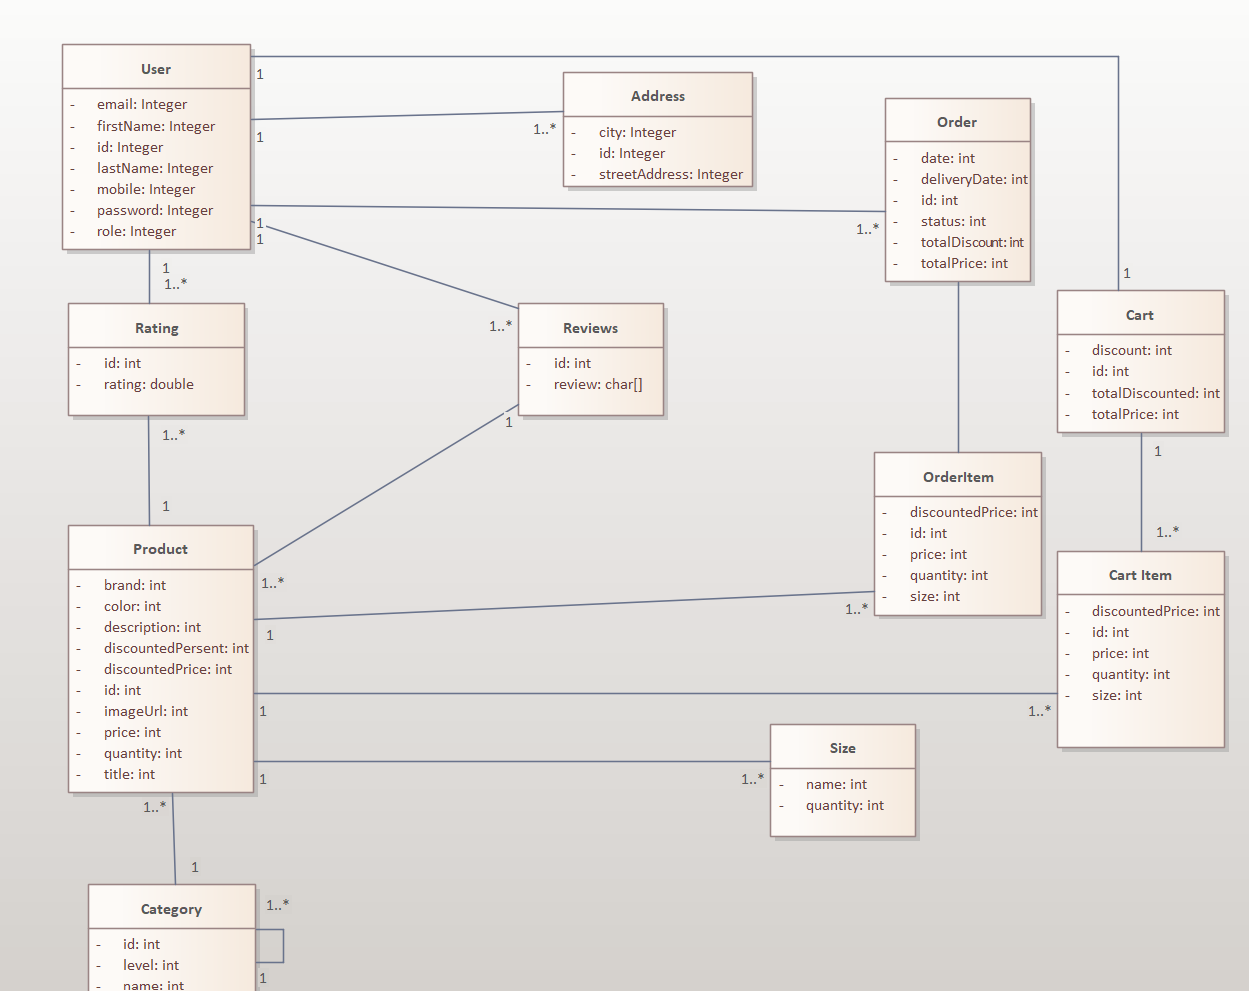
\includegraphics[width=15cm]{klassenDiagram.png}
	\caption{Klassendiagramm der Anwendung }
	\label{fig:klsdiag}
\end{figure}

\section{API-Dokumentation mit Swagger}
In diesem Abschnitt wird ein Ausschnitt der API-Dokumentation mithilfe von Swagger präsentiert. Das Swagger-UI bietet eine interaktive Darstellung der verfügbaren API-Endpunkte, ihrer Parameter und Rückgabewerte. Durch die Nutzung von Swagger können Entwickler die API-Funktionalität erkunden, testen und verstehen, ohne die Anwendung zu verlassen. Der folgende Screencap vermittelt einen Eindruck davon, wie die API mithilfe von Swagger dokumentiert ist und wie Benutzer mit den verschiedenen Endpunkten interagieren können.
\begin{figure}[H]
	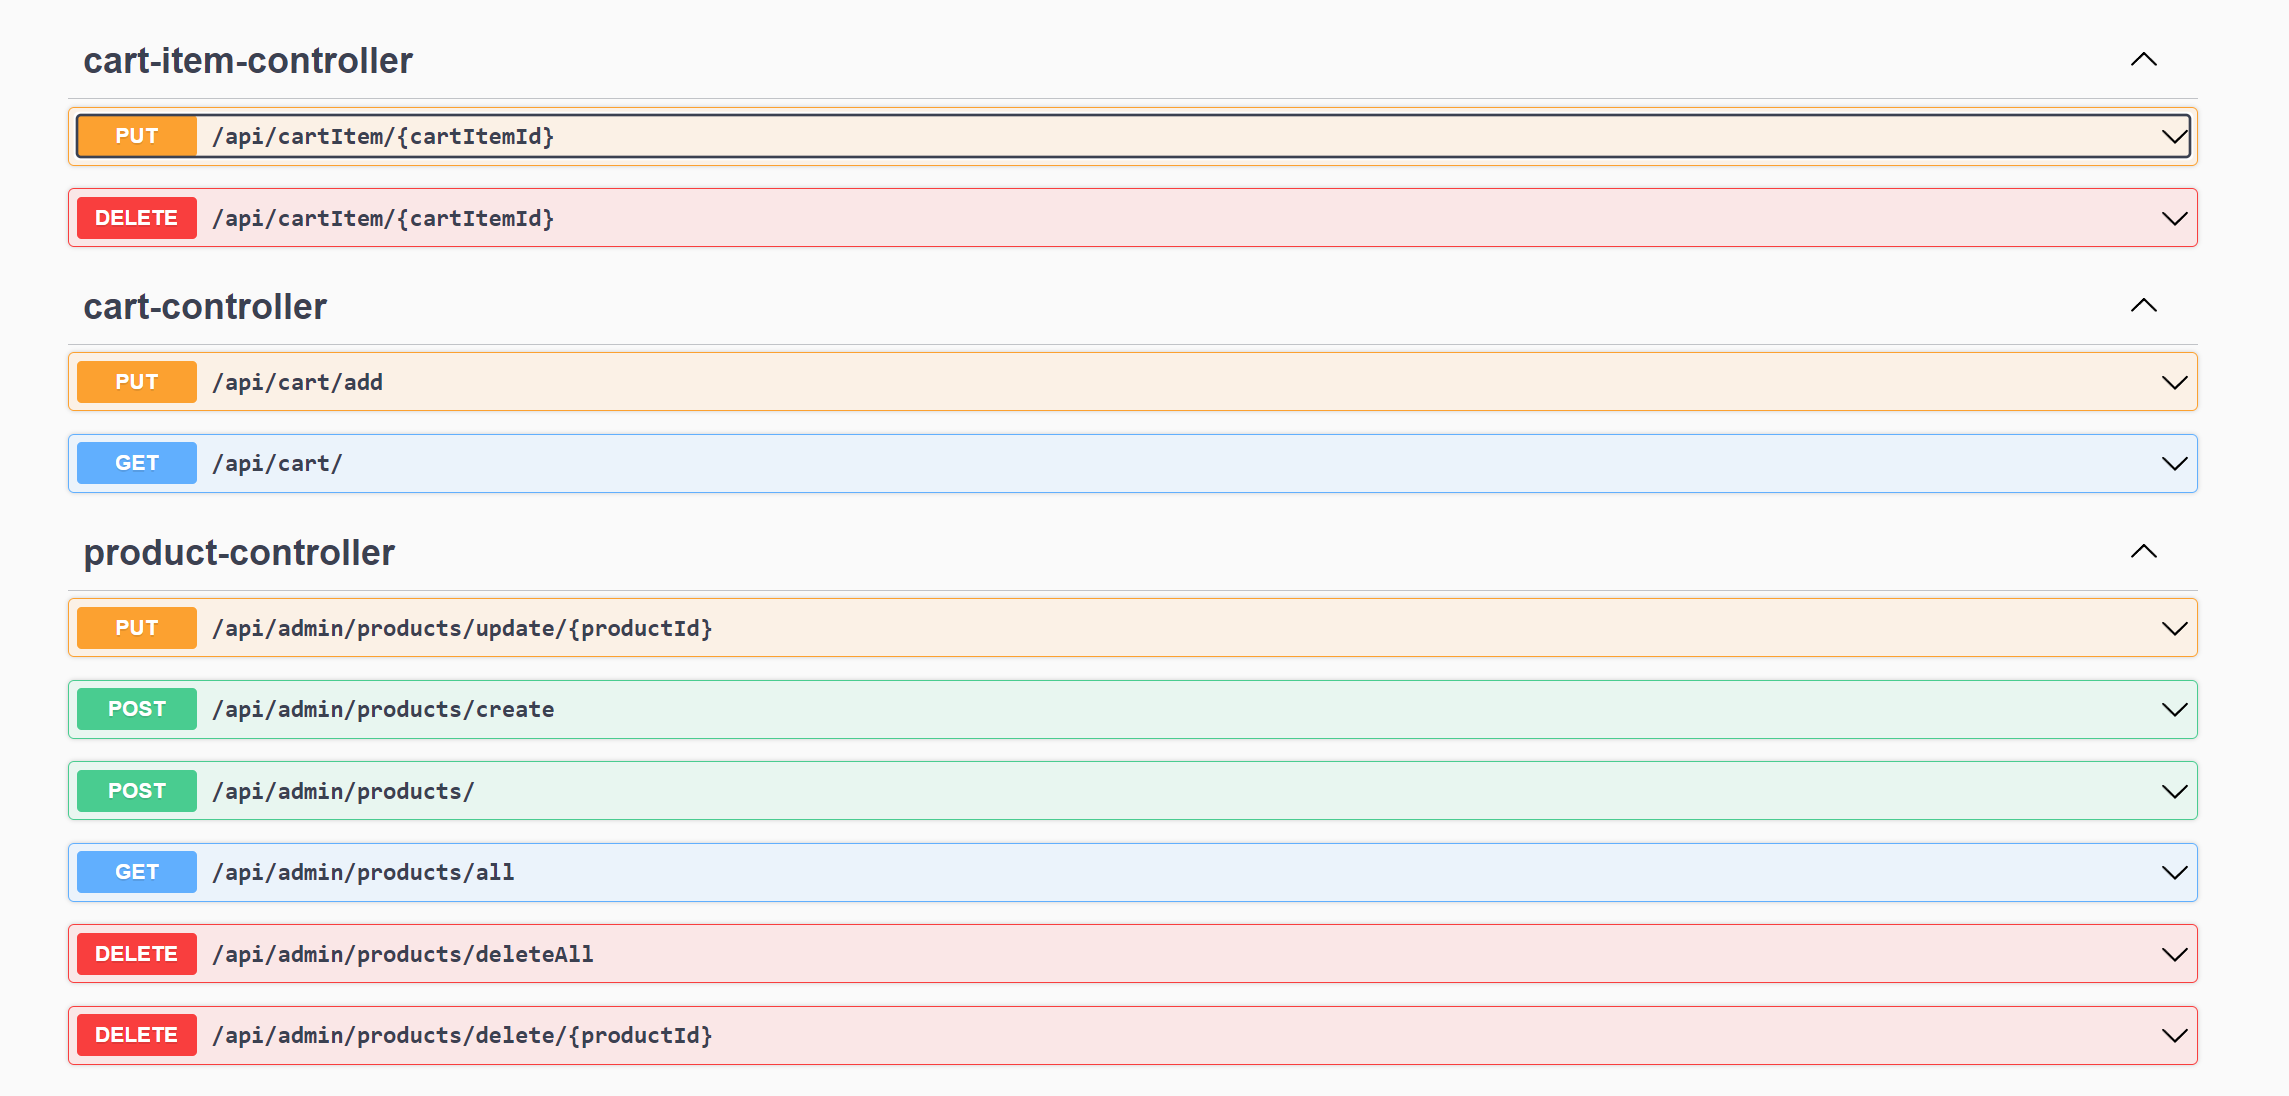
\includegraphics[width=17cm]{swagger1.png}
	\caption{Ausschnitt der API-Dokumentation 1 }
	\label{fig:swg1}
\end{figure}
\begin{figure}[H]
	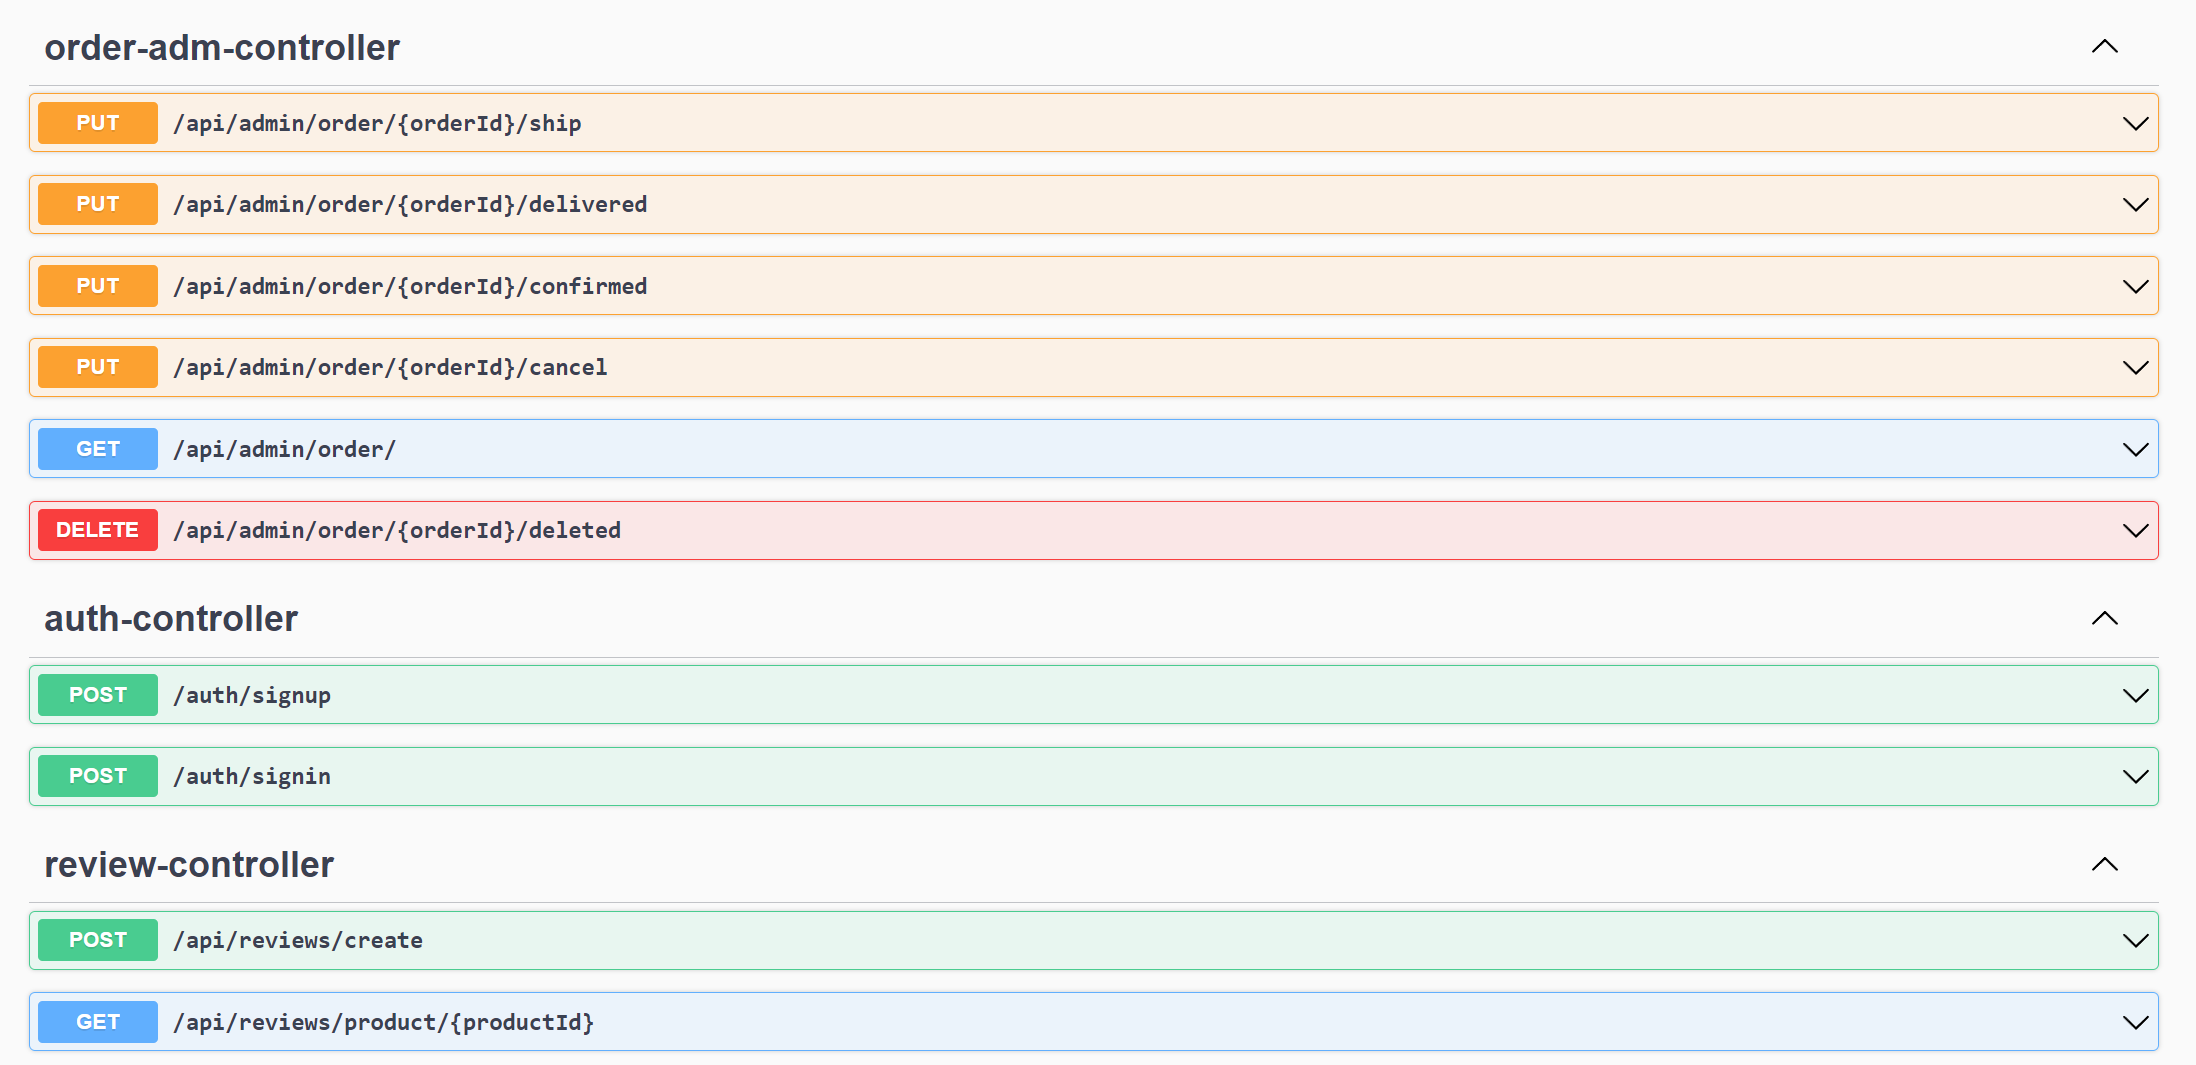
\includegraphics[width=17cm]{swagger2.png}
	\caption{Ausschnitt der API-Dokumentation 2 }
	\label{fig:swg2}
\end{figure}
\begin{itemize}
	
\item	\textbf{Authentifizierung:} Benutzer können sich mit JWT authentifizieren und Zugriff auf geschützte Ressourcen erhalten.
\item	\textbf{Produktsuche:} Kunden können Produkte nach bestimmten Kriterien suchen.
\item	\textbf{Warenkorb:} Kunden können Produkte hinzufügen und aus dem Warenkorb entfernen.
\item	\textbf{Bestellungen:} Kunden können Produkte aus dem Warenkorb bestellen.
\item	\textbf{Benutzerprofil:} Kunden können ihre Bestellungen einsehen. Darüber hinaus können sie Produktbewertungen und -rezensionen verfassen und hinzufügen.
\item	\textbf{Admin-Funktionen:} Der Administrator kann Produkte hinzufügen oder bearbeiten sowie Benutzerdaten ändern und Bestellungen einsehen.
	
\end{itemize}
	\chapter{Verwendete Technologien}
	Das Projekt nutzt eine Vielzahl von Technologien, die jeweils einem bestimmten Zweck dienen. Hier ist ein Überblick über die verwendeten Technologien:
	    \section{Backend-Entwicklung}
	\subsection{Java(Version 17.0.6 )} Verwendet als Backend-Programmiersprache für die Entwicklung der Anwendung. Java bietet eine robuste und zuverlässige Grundlage für die Implementierung der Geschäftslogik und Datenverarbeitung.
	\subsection{Spring Framework} Eingebunden für den Aufbau der Backend-Infrastruktur, einschließlich RESTful-Webdienste, Dependency Injection und MVC-Architektur.
	\subsubsection{Spring Boot (Version 3.2.2)}    
	Spring Boot bietet ein robustes und schlankes Framework für die Entwicklung von Java-basierten Anwendungen. Es vereinfacht die Konfiguration und den Aufbau von Anwendungen durch automatische Konventionen und Integrationen.
	
		\subsubsection{Spring Data (Version 3.2.2.)}
	Spring Data erleichtert Datenbankoperationen und die objektrelationale Abbildung (ORM) durch automatisierte Repository-Erstellung und Datenzugriffsmethoden.
	
	\subsubsection{Spring Web und Spring REST (Version 3.2.2)}
	Spring Web und Spring REST werden verwendet, um RESTful APIs zu erstellen und Webanfragen zu verarbeiten. Sie bieten Unterstützung für die Erstellung von RESTful Endpoints und die Verarbeitung von HTTP-Anfragen und -Antworten.
	

	
	\subsubsection{Spring Security (Version 6.2.1)}
	Spring Security gewährleistet die Authentifizierung und Autorisierung von Benutzern für einen sicheren Zugriff auf Ressourcen. Es bietet Funktionen wie Authentifizierung mit Benutzername/Passwort, OAuth, JWT usw.
	
	\subsubsection{Spring Validator (Version 3.0.2)}
	Spring Validator bietet Unterstützung für die Validierung von Dateninputs und die Sicherstellung der Datenintegrität. Es ermöglicht die Definition von Validierungsregeln für Formulardaten und Eingabefelder.
	
	\subsubsection{Spring Devtools (Version 2.5.4)}
	Spring Devtools bietet eine verbesserte Entwicklungserfahrung mit Funktionen wie automatischem Neustart der Anwendung, LiveReload und Hot Swapping. Es beschleunigt den Entwicklungsprozess und erhöht die Produktivität.
	
	\subsubsection{Lombok (Version 1.18.20)}
	Lombok vereinfacht die Java-Entwicklung, indem es automatisch Boilerplate-Code generiert. Es reduziert den Aufwand beim Schreiben von Getter, Setter, Konstruktoren und anderen häufig verwendeten Methoden.
	
	\subsubsection{Stripe (Version 20.62.0)}
	Stripe ist eine leistungsstarke Zahlungsabwicklungsplattform, die die Integration von Zahlungsfunktionen in Anwendungen erleichtert. Mit Stripe können Entwickler Zahlungen akzeptieren, verwalten und abwickeln, ohne komplexe Infrastruktur aufbauen zu müssen. Durch die Nutzung von Stripe können Entwickler Zeit sparen und sich auf die Kernfunktionen ihrer Anwendungen konzentrieren, während Stripe die Zahlungsabwicklung effizient und sicher abwickelt.
	
	
	\section{Front-End Entwicklung}
	\subsection{React.js (Version 18.2.0)}
	 Verwendet für die Entwicklung der Benutzeroberfläche der E-Commerce-Website. React bietet eine komponentenbasierte Architektur für die Erstellung interaktiver und reaktiver Benutzeroberflächen.
	 \subsection{Redux (5.0.1)}
	 Eingebunden zur Verwaltung des globalen Zustands der Anwendung. Redux ermöglicht eine zentrale Speicherung von Daten und erleichtert die Handhabung komplexer Anwendungsdaten.
	 \subsection{MUI : Material-UI (Version 5.15.6)}Verwendet für die Implementierung von vorgefertigten React-Komponenten im Material Design-Stil. Material-UI verbessert die Benutzererfahrung durch konsistente und ansprechende Benutzeroberflächenkomponenten
	 \subsection{Tailwind CSS (Version 3.4.1)} Eingesetzt für das Styling der Benutzeroberfläche. Tailwind CSS bietet nützliche CSS-Klassen, die eine schnelle Entwicklung und Anpassung von UI-Elementen ermöglichen.
	  \subsection{JavaScript / HTML / CSS / SCSS} Wesentliche Web-Technologien, die für
	 Client-seitiges Scripting, Strukturierung von Webinhalten und Styling.
	 \section{Datenbank-Management}
	 \subsection{MySQL}
	 Verwendet als relationales Datenbankmanagementsystem (RDBMS) für die Speicherung von Produktinformationen, Benutzerdaten, Bestelldetails und anderen relevanten Daten
	 \section{Weiter Technologien}
	 \subsection{Git}
	 Eingesetzt für die Versionskontrolle und Zusammenarbeit im Entwicklungsprozess.
	 \subsection{IDEs (Integrierte Entwicklungsumgebungen)}
	 In der Entwicklung unserer Anwendung habe ich Visual Studio für das Frontend und IntelliJ IDEA für das Backend mit Spring Boot eingesetzt. Diese bewährten integrierten Entwicklungsumgebungen boten uns eine benutzerfreundliche Plattform für das Codieren, Debuggen und Testen, was zu effizienter Entwicklung und hoher Anwendungsqualität führte.
	
	\appendix
	
	
	\makeatletter
	\@ifclassloaded{scrartcl}{\section*{Fazit}
		\addcontentsline{toc}{section}{\protect\numberline{}Fazit}}
	{\chapter*{Fazit}}
	\makeatother
	Zusammenfassend lässt sich sagen, dass das Ecommerce-Projekt sein Ziel, eine nahtlose und effiziente Plattform für den Online-Einkauf zu schaffen, erreicht hat. Durch die Integration fortschrittlicher Technologien und benutzerorientierter Designprinzipien bietet das Projekt eine umfassende Lösung für Kunden und Administratoren gleichermaßen.
	
	Für Kunden bietet die E-Commerce-Plattform eine benutzerfreundliche Oberfläche, die ein einfaches Browsen, eine einfache Produktauswahl und eine einfache Kaufabwicklung ermöglicht. Funktionen wie Registrierung, Anmeldung und Auftragsverfolgung verbessern das gesamte Einkaufserlebnis, während sichere Zahlungsgateways die Sicherheit und Zuverlässigkeit der Transaktionen gewährleisten.
	
	Administratoren profitieren von robusten Backend-Funktionen, einschließlich Bestandsverwaltung, Auftragsabwicklung und Kundensupport-Tools. Die Skalierbarkeit und Flexibilität des Systems ermöglicht eine einfache Anpassung an veränderte Geschäftsanforderungen.
	
	Durch Echtzeit-Analysen und Datenvisualisierung ermöglicht das Ecommerce-Projekt Unternehmen, fundierte Entscheidungen in Bezug auf Bestandsmanagement, Marketingstrategien und Kundenbindung zu treffen. Durch den Einsatz von Spitzentechnologien wie React, Redux und Spring Boot bietet die Plattform eine hohe Leistung und Reaktionsfähigkeit auf verschiedenen Geräten und Betriebssystemen.
	
	Im Wesentlichen stellt das Ecommerce-Projekt einen bedeutenden Fortschritt im Bereich des Online-Handels dar und bietet eine skalierbare, sichere und benutzerfreundliche Lösung für Unternehmen, die im digitalen Zeitalter erfolgreich sein wollen. Da sich die Technologie ständig weiterentwickelt, ist das Projekt bereit für weitere Verbesserungen und Innovationen, die die Zukunft des E-Commerce in Richtung größerer Effizienz, Nachhaltigkeit und Kundenzufriedenheit vorantreiben.

	\backmatter                     % keine Zählung der folgenden Kapitel
	
	
	
	
\end{document}

%%% Local Variables:
%%% mode: latex
%%% TeX-master: t
%%% TeX-engine: luatex
%%% ispell-local-dictionary: "deutsch8"
%%% End:



% der folgende Kommentar wird vom Emacs gebraucht, ist also ansonsten ohne
% Bedeutung!

%%% Local Variables:
%%% TeX-engine: luatex
%%% mode: latex
%%% TeX-master: t
%%% ispell-local-dictionary: "deutsch8"
%%% End:
